\PassOptionsToPackage{unicode=true}{hyperref} % options for packages loaded elsewhere
\PassOptionsToPackage{hyphens}{url}
%
\documentclass[ignorenonframetext,aspectratio=169]{beamer}
\usepackage{pgfpages}
\setbeamertemplate{caption}[numbered]
\setbeamertemplate{caption label separator}{: }
\setbeamercolor{caption name}{fg=normal text.fg}
\beamertemplatenavigationsymbolsempty
\usepackage{lmodern}
\usepackage{amssymb,amsmath}
\usepackage{ifxetex,ifluatex}
\usepackage{fixltx2e} % provides \textsubscript
\ifnum 0\ifxetex 1\fi\ifluatex 1\fi=0 % if pdftex
  \usepackage[T1]{fontenc}
  \usepackage[utf8]{inputenc}
  \usepackage{textcomp} % provides euro and other symbols
\else % if luatex or xelatex
  \usepackage{unicode-math}
  \defaultfontfeatures{Ligatures=TeX,Scale=MatchLowercase}
\fi
% use upquote if available, for straight quotes in verbatim environments
\IfFileExists{upquote.sty}{\usepackage{upquote}}{}
% use microtype if available
\IfFileExists{microtype.sty}{%
\usepackage[]{microtype}
\UseMicrotypeSet[protrusion]{basicmath} % disable protrusion for tt fonts
}{}
\IfFileExists{parskip.sty}{%
\usepackage{parskip}
}{% else
\setlength{\parindent}{0pt}
\setlength{\parskip}{6pt plus 2pt minus 1pt}
}
\usepackage{hyperref}
\hypersetup{
            pdfborder={0 0 0},
            breaklinks=true}
\urlstyle{same}  % don't use monospace font for urls
\newif\ifbibliography
% Prevent slide breaks in the middle of a paragraph:
\widowpenalties 1 10000
\raggedbottom
\setbeamertemplate{part page}{
\centering
\begin{beamercolorbox}[sep=16pt,center]{part title}
  \usebeamerfont{part title}\insertpart\par
\end{beamercolorbox}
}
\setbeamertemplate{section page}{
\centering
\begin{beamercolorbox}[sep=12pt,center]{part title}
  \usebeamerfont{section title}\insertsection\par
\end{beamercolorbox}
}
\setbeamertemplate{subsection page}{
\centering
\begin{beamercolorbox}[sep=8pt,center]{part title}
  \usebeamerfont{subsection title}\insertsubsection\par
\end{beamercolorbox}
}
\AtBeginPart{
  \frame{\partpage}
}
\AtBeginSection{
  \ifbibliography
  \else
    \frame{\sectionpage}
  \fi
}
\AtBeginSubsection{
  \frame{\subsectionpage}
}
\setlength{\emergencystretch}{3em}  % prevent overfull lines
\providecommand{\tightlist}{%
  \setlength{\itemsep}{0pt}\setlength{\parskip}{0pt}}
\setcounter{secnumdepth}{0}

% set default figure placement to htbp
\makeatletter
\def\fps@figure{htbp}
\makeatother

\DeclareUnicodeCharacter{00A0}{~}
\DeclareUnicodeCharacter{03B4}{$\delta$}
\DeclareUnicodeCharacter{03B5}{$\varepsilon$}
\DeclareUnicodeCharacter{03C9}{$\omega$}
\DeclareUnicodeCharacter{2124}{\mathbb{Z}}
\DeclareUnicodeCharacter{2193}{$\downarrow$}
\DeclareUnicodeCharacter{2208}{$\in$}
\DeclareUnicodeCharacter{2209}{$\notin$}
\DeclareUnicodeCharacter{220B}{$\ni$}
\DeclareUnicodeCharacter{2227}{$\wedge$}
\DeclareUnicodeCharacter{2228}{$\vee$}
\DeclareUnicodeCharacter{2234}{$\therefore$}
\DeclareUnicodeCharacter{2264}{$\leq$}
\DeclareUnicodeCharacter{2265}{$\geq$}
\DeclareUnicodeCharacter{2605}{$\star$}
\DeclareUnicodeCharacter{1D53D}{\mathbb{F}}


\hypersetup{colorlinks,linkcolor=,urlcolor=purple}
\setbeamertemplate{navigation symbols}{}
\usefonttheme[onlymath]{serif}

\title{\bf Clevis and Tang}
\providecommand{\subtitle}[1]{}
\subtitle{\bf Securing your secrets at rest}
\author{{\bf Fraser Tweedale}\\
    \texttt{@hackuador}\\
    \bigskip
    \def\svgwidth{4cm}
    \input{Logo-RedHat-A-Color-RGB-ARTIFACT.pdf_tex}}
\date{January 15, 2020}

\begin{document}
\frame{\titlepage}

\begin{frame}{~~}
\protect\hypertarget{section}{}

\begin{center}
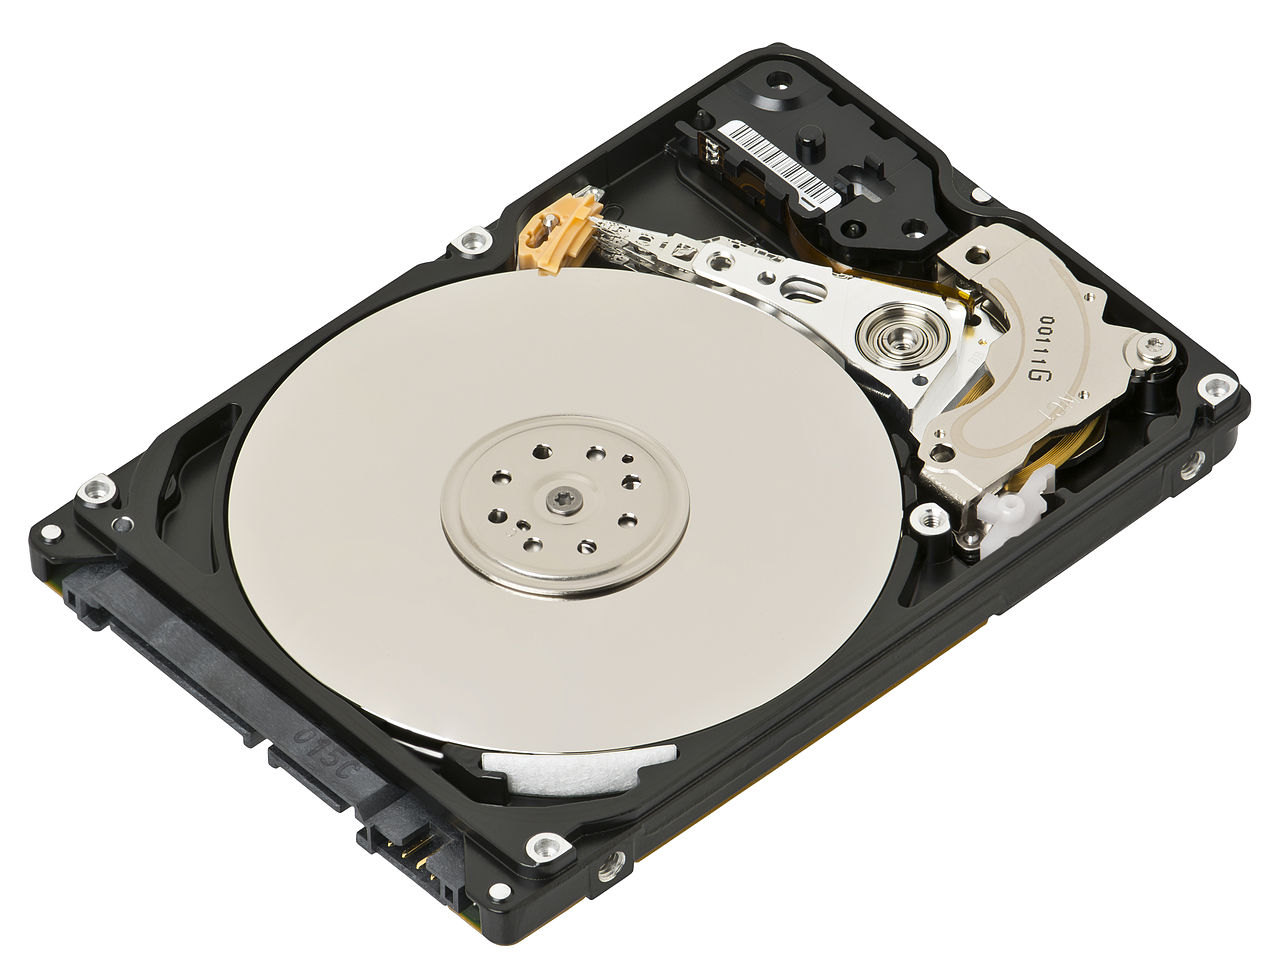
\includegraphics[width=.6\columnwidth]{Laptop-hard-drive-exposed.jpg}
\end{center}
\tiny

CC BY-SA 3.0
\url{https://commons.wikimedia.org/wiki/File:Laptop-hard-drive-exposed.jpg}

\end{frame}

\begin{frame}{~~}
\protect\hypertarget{section-1}{}

\begin{center}
\def\svgwidth{.5\paperheight}
\input{identity-secure-ARTIFACT.pdf_tex}
\end{center}

\end{frame}

\begin{frame}{~~}
\protect\hypertarget{section-2}{}

\begin{center}
\def\svgwidth{.6\columnwidth}
\input{USB_Icon-ARTIFACT.pdf_tex}
\end{center}

\end{frame}

\begin{frame}[plain]
\centering
\huge Demo
\end{frame}

\begin{frame}{Tang}
\protect\hypertarget{tang}{}

\begin{itemize}
\item Simple provisioning of encryption for secrets
\item Automated decryption when Tang server is available

  \begin{itemize}
  \item secret is \emph{``bound to the network''}
  \end{itemize}
\item
  Secret \textbf{never} leaves the client
\end{itemize}

\end{frame}

\begin{frame}{Tang - assumptions}
\protect\hypertarget{tang---assumptions}{}

\begin{itemize}
\item Tang server only accessible from ``secure network''
\item secrets and keys are safe in client memory
\item sufficient entropy at provisioning {\em and decryption}
\end{itemize}

\end{frame}

\begin{frame}[plain]
\begin{columns}
\column{\dimexpr\paperwidth}
  
\includegraphics[height=\paperheight]{caution.jpg}
\end{columns}
\end{frame}

\begin{frame}{Diffie-Hellman (DH) key agreement}
\protect\hypertarget{diffie-hellman-exchange}{}
\begin{itemize}
\normalsize
\item Alice and Bob agree on a \emph{shared secret}
\item Eve (the eavesdropper) cannot learn shared key
\item Parameters:
    \begin{itemize}
	\normalsize
	\item cyclic group \(G\) of order \(n\), with \emph{hard problem}
	  \begin{itemize}
	    \normalsize
	  \item \(ℤ^\times_p\) (discrete log)
	  \item elliptic curve \(E(𝔽_q)\) (point factorisation)
	  \end{itemize}
	\item generator \(g \in G\)
    \end{itemize}
\end{itemize}
\end{frame}

\item cyclic group \(G\) of order \(n\), with \emph{hard problem}
  \begin{itemize}
  \item \(ℤ^\times_p\) (discrete log)
  \item elliptic curve \(E(𝔽_q)\) (point factorisation)
  \end{itemize}
\item generator \(g \in G\)
\item key derivation function $KDF$ (e.g. SHA-256)
\item symmetric encryption algorithm \(Enc\) (e.g. AES-GCM)

\begin{frame}{Diffie-Hellman key agreement}
\protect\hypertarget{diffie-hellman}{}
\begin{center}
\def\arraystretch{1.5}%
\begin{tabular}{ l l l }
    ~ & \multicolumn{1}{c}{Client} & \multicolumn{1}{c}{Server} \\ \hline
    {\small 1.~~~~} & $A \in_R [1, n-1]$ & $B \in_R [1, n-1]$ \\
    {\small 2.~~~~} & $a \gets g^A$      & $b \gets g^B$ \\
    {\small 3.~~~~} & \multicolumn{2}{c}{$ a \to $} \\
                    & \multicolumn{2}{c}{$ \gets b $} \\
    {\small 4.~~~~} & $ K \gets b^A = g^{AB} $ & $ K \gets a^B = g^{AB} $ \\
\end{tabular}
\end{center}
\end{frame}

\begin{frame}{Integrated Encryption Scheme (IES)}
\protect\hypertarget{integrated-encryption-scheme}{}

\begin{itemize}
\item Encryption protocol based on Diffie-Hellman
\item Derive \emph{symmetric key} from shared secret
\item Alice encrypts a message to Bob's public key; sends it
\item Bob can decrypt the message, Eve cannot
\end{itemize}

\end{frame}

\begin{frame}{McCallum-Relyea exchange}
\protect\hypertarget{mccallum-relyea-exchange}{}

\begin{itemize}
\item Encryption protocol based on DH/IES

  \begin{itemize}
  \item due to Nathaniel McCallum and Robert Relyea:
	    \url{https://marc.info/?m=144173814525805}
  \end{itemize}
\item Alice encrypts to Bob's public key; \textbf{doesn't send message}
\item To decrypt, Alice asks Bob to encrypt an \emph{ephemeral key}

  \begin{itemize}
  \item uses reply to recover secret
  \end{itemize}
\item
  Eve cannot decrypt the message \textbf{\emph{and neither can Bob!}}
\end{itemize}

\end{frame}

\begin{frame}{McCallum-Relyea - parameters}
\protect\hypertarget{mccallum-relyea-parameters}{}
\begin{itemize}
\item $G$, $n$, $g \in G$ (same as DH)
\item key derivation function $KDF$ (e.g. SHA-256)
\item symmetric encryption algorithm \(Enc\) (e.g. AES-GCM)
\item message \(m\) to be encrypted
  \begin{itemize}
  \item e.g. content encryption key (CEK)
  \end{itemize}
\end{itemize}
\end{frame}

\begin{frame}{McCallum-Relyea - provisioning}
\protect\hypertarget{mccallum-relyea-provisioning}{}

\begin{center}
\def\arraystretch{1.5}%
\begin{tabular}{ l l l }
    ~ & \multicolumn{1}{c}{Client} & \multicolumn{1}{c}{Server} \\ \hline
    {\small 1.~~~~} & $A \in_R [1, n-1]$ & $B \in_R [1, n-1]$ \\
    {\small 2.~~~~} &                    & $b \gets g^B$ \\
    {\small 3.~~~~} & \multicolumn{2}{c}{$ \gets b $} \\
    {\small 4.~~~~} & $ K \gets KDF(b^A = g^{AB}) $ & \\
    {\small 5.~~~~} & $ a \gets g^A,~~~c \gets Enc(K, m) $ & \\
    {\small 6.~~~~} & $ \varnothing \gets A, K $ & \\
\end{tabular}
\end{center}

\end{frame}

\begin{frame}{McCallum-Relyea - decryption}
\protect\hypertarget{mccallum-relyea---decryption}{}

\begin{center}
\def\arraystretch{1.5}%
\begin{tabular}{ l l l }
  ~ & \multicolumn{1}{c}{Client} & \multicolumn{1}{c}{Server} \\ \hline
 {\small 1.~~~~} &  $X \in_R [1, n-1]$ & \\
 {\small 2.~~~~} &  $ x \gets a \cdot g^X = g^A \cdot g^X $ & \\
 {\small 3.~~~~} &  \multicolumn{2}{c}{$ x \to $} \\
 {\small 4.~~~~} &  & $x' \gets x^B = g^{AB} \cdot g^{XB} $ \\
 {\small 5.~~~~} &  \multicolumn{2}{c}{$ \gets x' $} \\
 {\small 6.~~~~} &  $ K \gets KDF(x' \cdot (b^X)^{-1}) $ & \\
        ~        &  $ ~~~ = KDF(g^{AB} \cdot g^{XB} \cdot g^{-XB}) = KDF(g^{AB}) $ & \\
 {\small 7.~~~~} &  $ m \gets Enc^{-1}(K, c) $ & \\
\end{tabular}
\end{center}

\end{frame}

\begin{frame}{Tang - implementation}
\protect\hypertarget{tang---implementation}{}

\begin{itemize}
\item
  Server-side daemon and \emph{Clevis pin}
\item
  C
\item
  Extensive test suite
\item
  Small and fast (\textgreater{}30k req/sec)
\end{itemize}

\end{frame}

\begin{frame}{Tang - protocol}
\protect\hypertarget{tang---protocol}{}

\begin{itemize}
\item JSON / JOSE objects over HTTP
\item No TLS (not needed)
\item Trust On First Use (TOFU)

  \begin{itemize}
  \item signed messages allow key rotation
  \end{itemize}

\item {\bf offline provisioning} is possible
\end{itemize}

\end{frame}

\begin{frame}{Tang - threats and caveats}
\protect\hypertarget{tang---threats-and-caveats}{}

\begin{itemize}
\item
  MitM during provisioning
\item
  Tang server is DoS target
\item
  Good entropy needed for ephemeral key \(X\)
\item
  Quantum computing (SIDH?)
\end{itemize}

\end{frame}

\hypertarget{mission-accomplished}{%
\section{Mission accomplished}\label{mission-accomplished}}

\hypertarget{section-3}{%
\section{???}\label{section-3}}

\begin{frame}{To what other things can we bind secrets?}
\protect\hypertarget{to-what-other-things-can-we-bind-secrets}{}
\begin{itemize}
\item Trusted Platform Module (TPM)
\item Smart Card
\item Bluetooth LE beacon ?
\item Escrowed key
\item Biometrics ???
\end{itemize}
\end{frame}

\begin{frame}{Unlock policy}
\protect\hypertarget{unlock-policy}{}
\begin{itemize}
\item Security is not binary
\item Policy should be driven by business needs (not tech)
\item How can we support arbitrarily complex unlock policy?
\end{itemize}
\end{frame}

\begin{frame}{Shamir's Secret Sharing}
\protect\hypertarget{shamirs-secret-sharing}{}

\begin{itemize}
\item
  \(k\) points describe a polynomial of degree \(k - 1\)
\item
  Free coefficient \(\gets\) secret, other coefficients \(\gets_R\)
\item
  Distribute \(n\) points (\(n \ge k, x \ne 0\))
\item
  Given \(k\) points, compute \emph{Lagrange polynomial}

  \begin{itemize}
  \item
    secret \(\gets f(0)\)
  \end{itemize}
\end{itemize}

\end{frame}

\begin{frame}{Shamir's Secret Sharing}
\protect\hypertarget{shamirs-secret-sharing-plot}{}

\begin{center}
\def\svgwidth{.8\columnwidth}
\input{Lagrange_polynomial-ARTIFACT.pdf_tex}
\end{center}
\tiny

CC BY-SA 3.0
\url{https://en.wikipedia.org/wiki/File:Lagrange_polynomial.svg}

\end{frame}

\begin{frame}[plain]
\begin{columns}
\column{\dimexpr\paperwidth}
  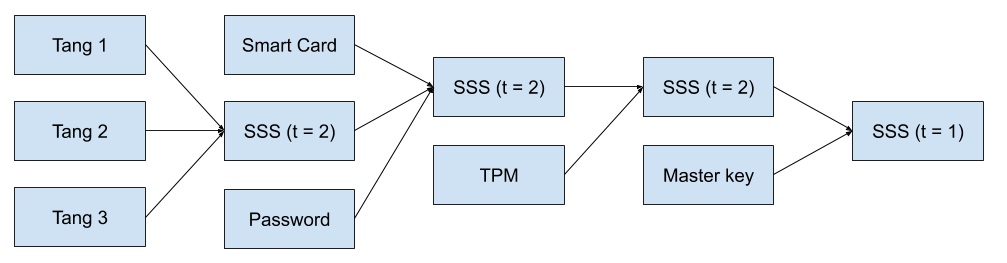
\includegraphics[width=\textwidth]{policy.png}
\end{columns}
\end{frame}

\begin{frame}{Clevis}
\protect\hypertarget{clevis}{}

\begin{itemize}
\item Client-side, pluggable key management based on SSS
\item
  \emph{pins} (plugins)

  \begin{itemize}
  \item {\tt tang}, {\tt tpm2}, {\tt sss}, ...
  \end{itemize}
\item
  JSON configuration
\item
  C
\end{itemize}

\end{frame}

\begin{frame}[plain]
\centering
\huge Demo
\end{frame}

\begin{frame}{LUKS integration}
\protect\hypertarget{luks-integration}{}

\begin{itemize}
\item \emph{Linux Unified Key Setup}
\item LUKS (v1): Tang only
\item LUKS 2: {\bf full Clevis support}
  \begin{itemize}
  \item dracut, systemd and udisks2 unlockers
  \item {\tt clevis-luks-unlockers(7)}
  \end{itemize}
\end{itemize}

\end{frame}


\begin{frame}{History}
\protect\hypertarget{history}{}

\begin{itemize}
\item Feb '15: \emph{Deo} project begins (\emph{δεω, to bind})

  \begin{itemize}
  \item Used TLS for privacy and X.509 encryption cert (\emph{complexity!})
  \item Server decrypts and returns secret (thus learning it; \emph{bad!})
  \end{itemize}
\item Sep '15: McCallum-Relyea discovered; rewrite begins
\item Dec '15: Project split into Tang and Clevis
\end{itemize}

\end{frame}

\begin{frame}[fragile]{Availability}
\protect\hypertarget{availability}{}

\begin{itemize}
\item Fedora ≥ 24
\item RHEL ≥ 7.4
\item Debian ≥ 10 (buster)
\item Ubuntu ≥ 18.04 LTS (bionic)
\item Source code (GPLv3+)

  \begin{itemize}
  \item \url{https://github.com/latchset/tang}
  \item \url{https://github.com/latchset/clevis}
  \end{itemize}
\end{itemize}

\end{frame}

\begin{frame}{You can help!}
\protect\hypertarget{you-can-help}{}

\begin{itemize}
\item Try it (+ file bugs)
\item Explain your use cases
\item Contribute Clevis pins
\item Implement for other OSes
\item Publish blog posts / tutorials / demos
\end{itemize}

\end{frame}

\begin{frame}[plain]
\begin{columns}

  \begin{column}{.4\textwidth}
    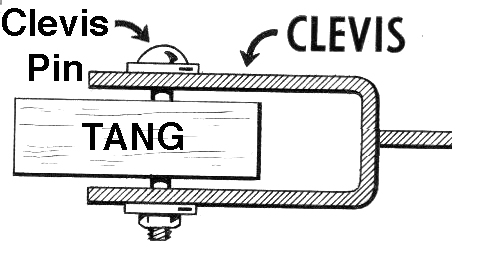
\includegraphics[width=1.2\textwidth]{clevis.jpg}

\begin{center}
\href{https://access.redhat.com/documentation/en-us/red_hat_enterprise_linux/8/html/security_hardening/configuring-automated-unlocking-of-encrypted-volumes-using-policy-based-decryption_security-hardening}{RHEL documentation}
\\
\smallskip
\url{https://github.com/latchset}
\end{center}

  \end{column}

  \begin{column}{.6\textwidth}

    \setlength{\parskip}{.5em}

    { \centering

    \input{cc-by-ARTIFACT.pdf_tex}

    \copyright~2020  Red Hat, Inc.

    { \scriptsize
    Except where otherwise noted this work is licensed under
    }
    { \footnotesize
    \textbf{http://creativecommons.org/licenses/by/4.0/}
    }

    }

    \begin{description}
      \item[Slides] \href{https://speakerdeck.com/frasertweedale}{speakerdeck.com/frasertweedale}
      \item[Blog] \href{https://frasertweedale.github.io/blog-redhat/}{frasertweedale.github.io/blog-redhat}
      \item[Email] \texttt{ftweedal@redhat.com}
      \item[Twitter] \href{https://twitter.com/hackuador}{@hackuador}
    \end{description}
  \end{column}

\end{columns}
\end{frame}

\end{document}
